\documentclass[11pt,letterpaper]{report}
\usepackage[utf8]{inputenc}
\usepackage[left=1in,right=1in,top=1in,bottom=1in]{geometry}
\usepackage{amsfonts,amsmath}
\usepackage{graphicx,float}
\usepackage{titlesec}
\usepackage{csquotes}
\usepackage{esint}
% -----------------------------------
\usepackage{hyperref}
\hypersetup{%
  colorlinks=true,
  linkcolor=blue,
  citecolor=blue,
  urlcolor=blue,
  linkbordercolor={0 0 1}
}
% -----------------------------------
\usepackage[style=authoryear-icomp,backend=biber]{biblatex}
\addbibresource{citation.bib}
% -----------------------------------
\setlength{\parindent}{0.0in}
\setlength{\parskip}{0.1in}
% -----------------------------------
\newcommand{\de}{\mathrm{d}}
\newcommand{\DD}{\mathrm{D}}
\newcommand{\pe}{\partial}
\newcommand{\mcal}{\mathcal}
%\newcommand{\pdx}{\left|\frac{\partial}{\partial_x}\right|}

\newcommand{\dsp}{\displaystyle}

\newcommand{\norm}[1]{\left\Vert #1 \right\Vert}
%\newcommand{\mean}[1]{\left\langle #1 \right\rangle}
\newcommand{\mean}[1]{\overline{#1}}
\newcommand{\inner}[2]{\left\langle #1,#2\right\rangle}

\newcommand{\ve}[1]{\boldsymbol{#1}}

\newcommand{\thus}{\Rightarrow \quad }
\newcommand{\fff}{\iff\quad}
\newcommand{\qdt}[1]{\quad \mbox{#1} \quad}

\renewcommand{\Re}{\mathrm{Re}}
\renewcommand{\Im}{\mathrm{Im}}
\newcommand{\E}{\mathbb{E}}
\newcommand{\lap} {\nabla^2}
\renewcommand{\div}{\nabla\cdot}

\newcommand{\csch}{\text{csch}}
\newcommand{\sech}{\text{sech}}


\newcommand{\hot}{\text{h.o.t.}}

\newcommand{\ssp}{\left.\qquad\right.}

\newcommand{\var}{\text{var}}
\newcommand{\cov}{\text{cov}}


% -----------------------------------
\renewcommand\thesection{\arabic{chapter}.\arabic{section}}
\renewcommand\thesubsection{(\arabic{section}.\alph{subsection})}
  
\titleformat{\subsection}[runin]
        {\normalfont\bfseries}
        {\thesubsection}% the label and number
        {0.5em}% space between label/number and subsection title
        {}% formatting commands applied just to subsection title
        []% punctuation or other commands following subsection title
% -----------------------------------
\begin{document}
\begin{titlepage}
    \begin{center}
        \vspace*{4cm}
        \Huge
        \textbf{Recitation Materials} \\
        \vspace{0.5cm}
        \LARGE
        {for NYU Undergraduate Introduction To Fluid Dynamics}\\
        \vspace{3cm}
        By\\
        \vspace{0.5cm}
        \textbf{Ryan Sh\`iji\'e D\`u}\\
        \vspace{0.2cm}
        \normalsize
        {Courant Institute of Mathematical Sciences - New York University}\\
        \vspace{2cm}
        \Large
        \textbf{Spring, 2023}
        
    \end{center}
\end{titlepage}

\setcounter{tocdepth}{1}
\tableofcontents

\setcounter{chapter}{-1}
% -----------------------------------
\chapter{Before the Course Materials}
%\addcontentsline{toc}{chapter}{READ ME}
%\phantomsection
\section{READ ME}
This document is a compilation of the worksheets used in the recitation sessions for \href{https://math.nyu.edu/dynamic/courses/undergrad/math-ua-230/}{NYU Undergraduate Introduction To Fluid Dynamics} in Spring of 2023. We did not do all problems in this documents in class.

The \LaTeX\ files of this document can be found at \url{https://github.com/Empyreal092/UgradFluids_Worksheet}.

% For students in my recitations: the problems marked with *** are not in the weekly version of the worksheets. They are extra problems.

\chapter{Flow Kinematics}
\section{Rate of strain tensor: examples}
\subsection{Shear flow}
Take a velocity field with $u=y$ and $v,w=0$. 
\begin{enumerate}
    \item Calculate its velocity gradient tensor.
    \item What is its symmetric and anti-symmetric parts?
    \item What is its divergence and vorticity vector? 
\end{enumerate}

\subsection{Straining flow}
Take a velocity field with $u=x$, $v=-y$, and $w=0$. 
\begin{enumerate}
    \item Do the same calculation.
    \item {[Adapted from \cite{Aris_62}, Exercise 4.42.1]} Take a line connecting the origin and a fluid parcel, show that if $\theta$ is the angle between the line and the $x$-axis, then the rate of change of $\log\tan\theta$ is constant along a particle path. 
\end{enumerate}

\subsection{}
[From \cite{Aris_62}, Exercise 4.45.1] Take the velocity field
\begin{align}
    \ve v = \alpha\ve \omega + \ve \omega \times \ve x.
\end{align}
\begin{enumerate}
    \item Do the same calculation.
    \item Interpret the motion of a fluid parcel in this flow.
\end{enumerate}

\subsection{Rankine vortex}
Now we use the cylindrical coordinate with $(r,\theta,z)$. We have the flow field
\begin{align}
    u_\theta = \begin{cases}
        \Omega r, & r<a\\
        \dsp{\frac{\Omega a^2}{r}}, & r\geq a
    \end{cases}
\end{align}
and $u_r = u_z = 0$. 
\begin{enumerate}
    \item Do the same calculation (by converting the velocity into the Cartesian coordinate).
\end{enumerate}
We will come back to this example to practice polar coordinate and to study vorticity and circulation.  

\section{From divergence theorem to Green's theorem}
\subsection{}
[From \cite{Aris_62}, Exercise 3.31.3] By taking $\ve a$ to be independent of $x$, and $a_3 = 0$, show using divergence theorem that if $A$ is an area in the $(x,y)$-plane bounded by a curve $C$, then
\begin{align}
    \iint_A \frac{\pe a_1}{\pe x}+\frac{\pe a_2}{\pe y}\;\de A = \oint_C a_1t_2-a_2t_1\;\de s
\end{align}
where $\ve t=(t_1,t_2)$ is the unit tangent vector to $C$. 

\subsection{}
[From \cite{Aris_62}, Exercise 3.31.4] Deduce from the previous question that
\begin{align}
    \iint_A \frac{\pe a_2}{\pe x}-\frac{\pe a_1}{\pe y}\;\de A = \oint_C a_1t_1+a_2t_2\;\de s
\end{align}
The right hand side can be written as
\begin{align}
    \oint_C a_1\de x+a_2\de y
\end{align}
and we have derived the Green's theorem.

\section{Green's identity}
\subsection{}
We take a 3D scalar field $\psi$ and a 3D vector field $\ve\Gamma$ with sufficient smoothness defined on some region $U \subset \mathbb{R}^3$. Show the identity
\begin{align}
    \iiint_U \left( \psi \, \nabla \cdot \ve{\Gamma} + \ve{\Gamma} \cdot \nabla \psi\right)\, dV  = \oiint_{\partial U} \psi \left( \ve{\Gamma} \cdot \ve{n} \right)\, dS=\oiint_{\partial U}\psi\ve{\Gamma}\cdot d\ve{S}.\label{eq:green_1st_gen}
\end{align}

\subsection{}
Use \eqref{eq:green_1st_gen} to show the Green's first identity. Take 3D scalar fields $\psi$ and $\varphi$ both with sufficient smoothness:
\begin{align}
    \iiint_U \left( \psi \, \nabla^2 \varphi + \nabla \psi \cdot \nabla \varphi \right)\, dV  = \oiint_{\partial U} \psi \left( \nabla \varphi \cdot \ve{n} \right)\, dS=\oiint_{\partial U}\psi\,\nabla\varphi\cdot d\ve{S}.
\end{align}

\subsection{}
Show the Green's second identity:
\begin{align}
    \iiint_U \left( \psi \, \nabla^2 \varphi - \varphi \, \nabla^2 \psi\right)\, dV = \oiint_{\partial U} \left( \psi \nabla \varphi - \varphi \nabla \psi\right)\cdot d\ve{S}.
\end{align}
This shows that the Laplacian is a self-adjoint operator for functions vanishing on the boundary so that the right hand side of the above identity is zero.


% \section{Expanding gas}
% \subsection{In a tube}
% We have a velocity field $u=x$ and $v,w=0$. 
% \begin{enumerate}
%     \item Write down the ``differential form'' of the mass conservation equation.
%     \item Use the method of characteristic to solve for the density $\rho(x,t)$.
% \end{enumerate}

% \subsection{In free 3D space}
% Now have a velocity field $u=x$, $v=y$, and $w=z$. Do the same calculation.

\section{Deformation tensor: examples}
\subsection{Straining flow}
Take a velocity field with $u=x$, $v=-y$, and $w=0$. 
\begin{enumerate}
    \item Calculate the deformation tensor $\ve F$.
    \item Verify the Lagrangian equation of evolution for $\ve F$
        \begin{align}
            \left.\frac{\pe\ve F}{\pe t}\right|_{\ve\alpha} = \nabla_{\ve x}\ve v\cdot \ve F.
        \end{align}
\end{enumerate}

\subsection{}
Take a velocity field with $u=2x^{1/2}$, $v=2y^{1/2}$, and $w=2z^{1/2}$. 
\begin{enumerate}
    \item Do the same calculation.
    \item Also verify the Eulerian equation of evolution for $\ve F$:
        \begin{align}
            \left.\frac{\pe\ve F}{\pe t}\right|_{\ve x}+(\ve v\cdot\nabla_{\ve x})\ve F = \nabla_{\ve x}\ve v\cdot \ve F.\label{eq:F_eq_euler}
        \end{align}
\end{enumerate}

\section{Evolution of an infinitesimal material line element}
Take an infinitesimal material line element $\delta\ve \ell$, where it is the
infinitesimal material element connecting $\ve\ell$ and $\ve\ell+\delta\ve\ell$. Show that its evolution equation follows the equation
\begin{align}
    \frac{D\delta\ve\ell}{Dt}=\nabla_{\ve x}\ve v\cdot \delta\ve\ell.
\end{align}
You will do this in the homework using \eqref{eq:F_eq_euler}. I want you to think about it from another perspective: use your physical intuition and argue using infinitesimal time. 

Hint: local in time, the velocity at $\ve\ell$ is $\ve v$ and the velocity at $\ve\ell+\delta\ve\ell$ is $\ve v+\delta\ve v$. What is $\delta\ve v$?

\chapter{Euler Equations}
\section{Derivation of the Lamb vector}
A useful vector identity in fluid mechanics is
\begin{align}
    \ve v(\nabla\cdot\ve v) = \frac{1}{2}\nabla\ve v^2-\ve v\times\ve \omega.\label{eq:lamb_ident}
\end{align}
For example, we use this identity in the derivation of the Bernoulli's principle. The Lamb vector is defined as
\begin{align}
    \ve\ell = \ve v\times\ve \omega.
\end{align}
We will derive the the vector identity \eqref{eq:lamb_ident}.

\subsection{}
Show that the cross product can be written as
\begin{align}
    \ve a\times \ve b = \epsilon_{ijk}a_ib_j\ve e_{(k)}
\end{align}
where $\epsilon_{ijk}$ is the permutation symbol:
\begin{align}
    \epsilon_{ijk} = \begin{cases}
        0 &\text{, if any two of $i,j,k$ are the same}\\
        1 &\text{, if $i,j,k$ is an even permutation of $1,2,3$}\\
        -1 &\text{, if $i,j,k$ is an odd permutation of $1,2,3$}.
    \end{cases}
\end{align}

\subsection{}
[From \cite{Aris_62}, Exercise 2.32.1] Show by enumerating typical cases that
\begin{align}
    \epsilon_{ijk}\epsilon_{k\ell m} = \delta_{i\ell}\delta_{jm}-\delta_{im}\delta_{j\ell}.\label{eq:perm_prod_ident}
\end{align}

\subsection{}
Use \eqref{eq:perm_prod_ident} to show \eqref{eq:lamb_ident}.

\section{Bernoulli's principle: examples}
\subsection{Flow out of a water tank}
Imagine a water tank with height $h$ of water inside. At the bottom there is a small hole. What would be the speed of the water flowing out of the hole.

\subsection{Venturi effect}
Calculate the fluid velocity difference at point 1 and 2 as a function of $h$.

Image from Wikipedia for Venturi effect. It is best to extend the lower end of the two vertical tubes to the center of the horizontal tube so that they stop at point 1 and 2.
\begin{figure}[H]
    \centering
    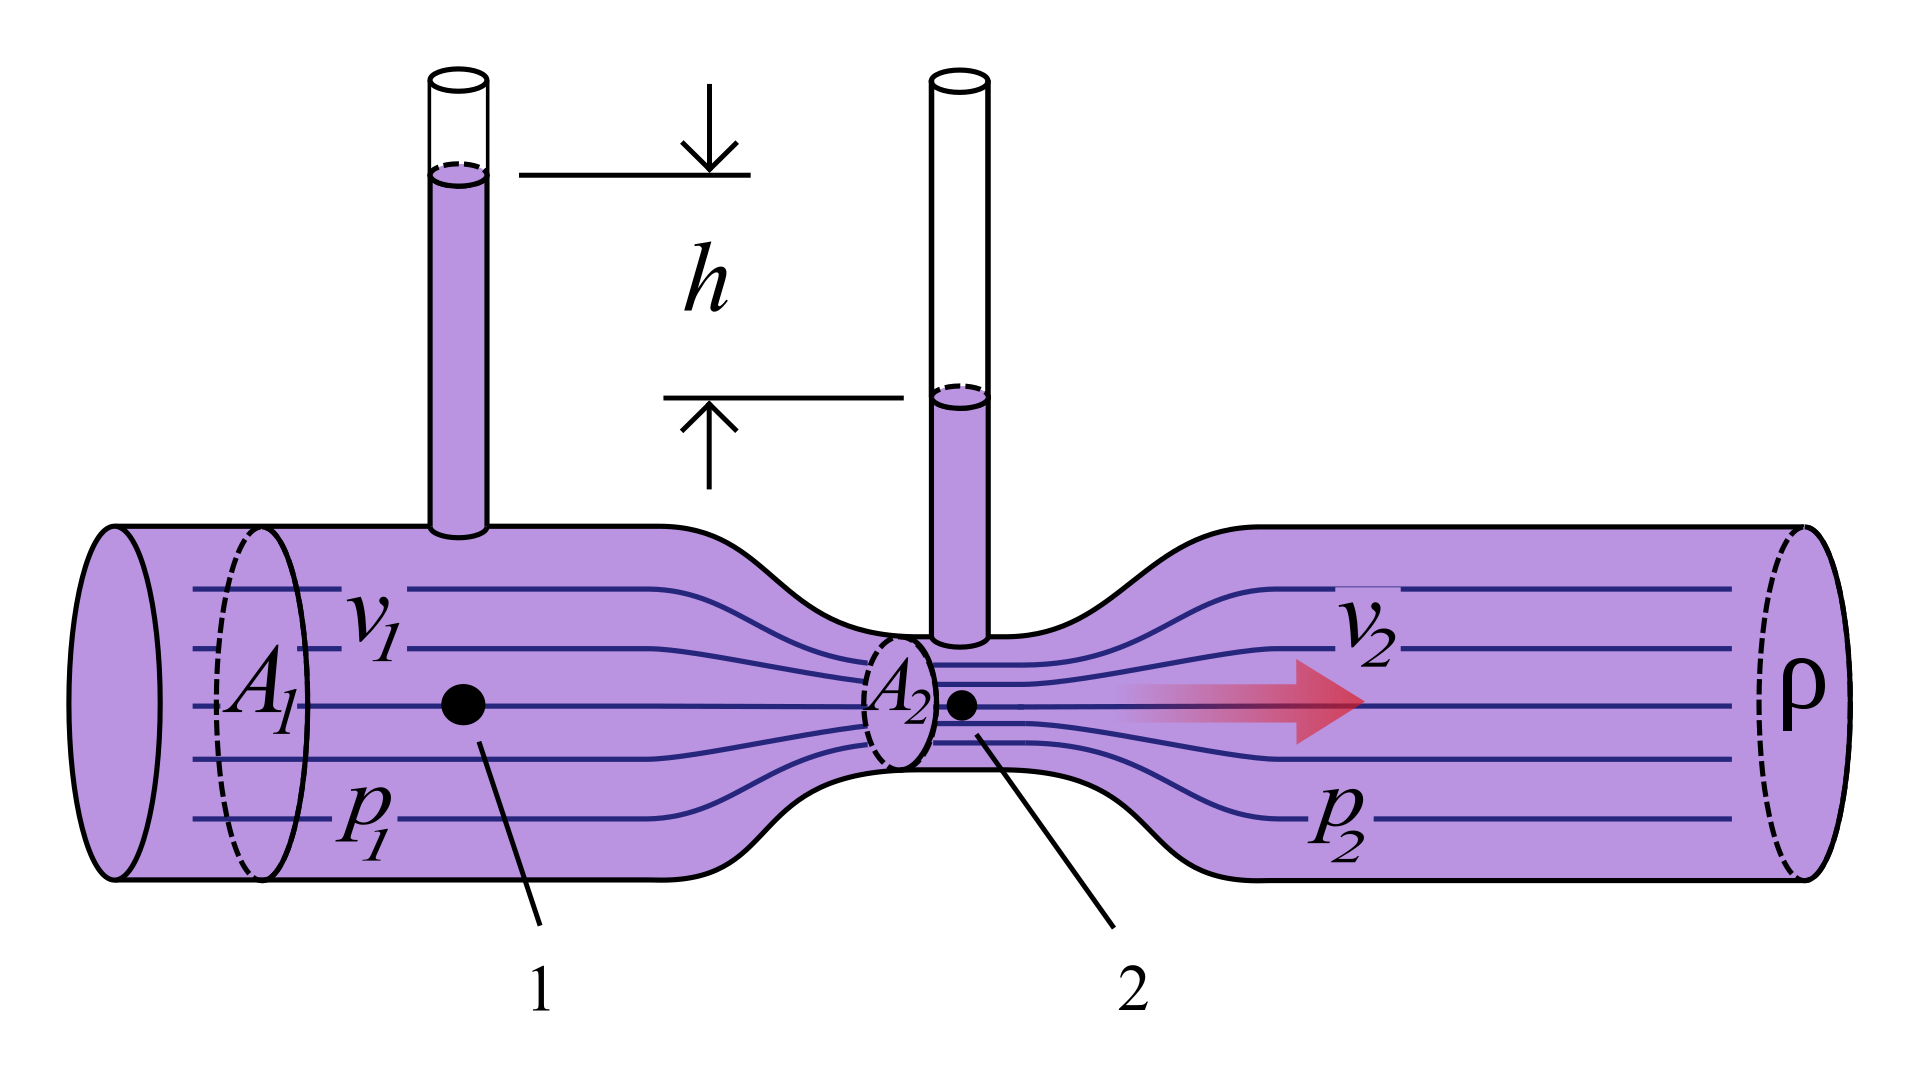
\includegraphics[width=0.5\textwidth]{Session_4/figs/Venturi_wiki}
\end{figure}

\subsection{Pitot's tube}
Using the idea of the above device, think of a device that measures the speed of the fluid flow.

\subsection{Lift on an airfoil: a first look}
Use Bernoulli's principle to explain how lift is generated by a plane's wing.

Image generated by Wolfram software from \url{https://demonstrations.wolfram.com/JoukowskiAirfoilFlowField/}. The lines are streamlines, the color is the pressure field.
\begin{figure}[H]
    \centering
    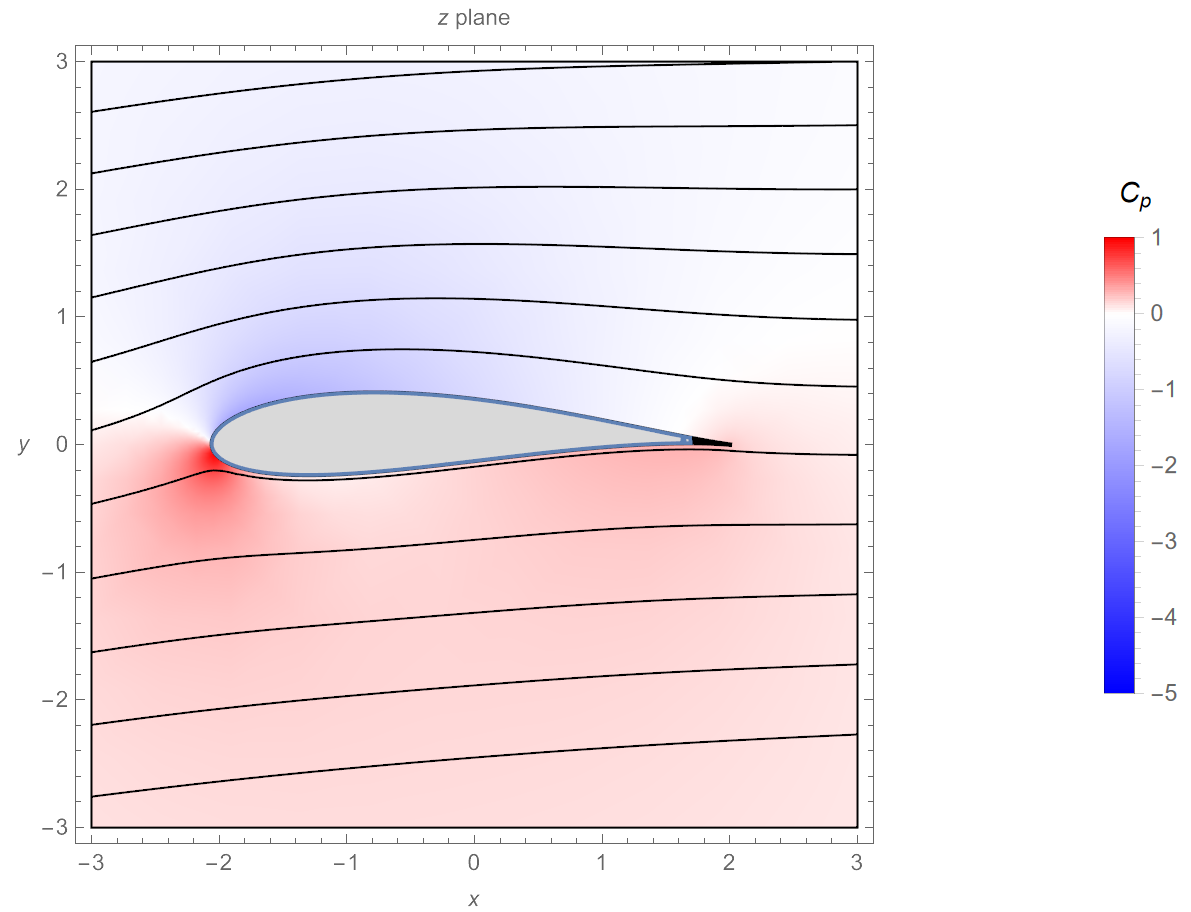
\includegraphics[width=0.6\textwidth]{Session_4/figs/Airfoil}
\end{figure}

\section{The ABC flows}
By using \eqref{eq:lamb_ident}, we can write the incompressible Euler equation as
\begin{align}
    &\frac{\pe\ve v}{\pe t}+\ve\omega\times\ve v = -\nabla H,\\
    &\nabla\cdot\ve v = 0.
\end{align}
where $H$ is the energy
\begin{align}
    H = \frac{p}{\rho}+\frac{1}{2}\ve v^2.
\end{align}
The Arnold, Beltrami, Childress (ABC) flow is an interesting steady state solution of Euler. It has the velocity field on the $2\pi$-periodic 3D domain
\begin{align}
    \begin{cases}
        u= A\sin z+C\cos y\\
        v= B\sin x+A\cos z\\
        w= C\sin y+B\cos x\\
    \end{cases}
\end{align}
where $A,B$, and $C$ are constant parameters. Despite its simple appearance in the Eulerian frame, the Lagrangian behavior of this flow is presumably chaotic. To quote \cite{DombreEtAl_86} which named this flow
\begin{displayquote}
Three-dimensional steady flows with a simple Eulerian representation can have a chaotic Lagrangian structure. By this we mean that infinitesimally close fluid particles following the streamlines may separate exponentially in time, while remaining in a bounded domain, and that individual streamlines may appear to fill entire regions of space.
\end{displayquote}
and
\begin{displayquote}
    From a fluid dynamical viewpoint flows with chaotic streamlines are interesting because they may considerably enhance transport without being turbulent in the usual sense - they only display what might be called `Lagrangian turbulence'.
\end{displayquote}

We will be less ambitious and show some basic properties of this flow.
\subsection{}
Show the ABC flows are incompressible.

\subsection{}
Show the ABC flows are Beltrami flows. That is
\begin{align}
    \ve \omega\times\ve v = 0.
\end{align}
Hint: Show $\ve \omega = \ve v$. Why does this identity shows $\ve v$ is Beltrami?

\subsection{}
Conclude the ABC flows are exact solution to the steady state incompressible Euler equation.

\chapter{Navier–Stokes Equations}
\section{Taylor–Green vortex}
The Taylor–Green vortex is an exact solution to the 2D Navier-Stokes equation:
\begin{align}
    &\frac{\partial u}{\partial t} + u\frac{\partial u}{\partial x} + v\frac{\partial u}{\partial y} = -\frac{1}{\rho} \frac{\partial p}{\partial x} + \nu \left( \frac{\partial^2 u}{\partial x^2} + \frac{\partial^2 u}{\partial y^2} \right),\\
    &\frac{\partial v}{\partial t} + u\frac{\partial v}{\partial x} + v\frac{\partial v}{\partial y} = -\frac{1}{\rho} \frac{\partial p}{\partial y} + \nu \left( \frac{\partial^2 v}{\partial x^2} + \frac{\partial^2 v}{\partial y^2} \right),\\
    &\frac{\partial u}{\partial x}+ \frac{\partial v}{\partial y} = 0.
\end{align}
The first appearance of this flow is in \cite{Taylor_23}. The name of this flows comes from the joint work \cite{TaylorGreen_37}. A 3D extension of the Taylor–Green vortex appeared recently in \cite{Antuono_20}. The exact solutions to the fluid equations are important tools for benchmarking numerical solvers for fluids dynamics. 

\subsection{}
The Taylor–Green vortex has velocity
\begin{align}
    u &= \cos x\sin y F(t)\\
    v &= -\sin x\cos y F(t).
\end{align}
Show, by plugging the velocity into the momentum equation, that the pressure field is given by
\begin{align}
    p = -\frac{\rho}{4}(\cos 2x+\cos 2y)F^2(t).
\end{align}

\subsection{}
Now show that the time component is
\begin{align}
    F(t) = e^{-2\nu t}.
\end{align}

\section{Alternative form for momentum dissipation}
\subsection{}
[From \cite{Aris_62}, Exercise 3.24.5] Show the vector identity
\begin{align}
    \nabla^2 \ve v = \nabla(\nabla\cdot\ve v)-\nabla\times(\nabla\times \ve v).
\end{align}

\subsection{}
[From \cite{Aris_62}, \S 6.11] Show that the incompressible Navier-Stokes can alternatively be written as
\begin{align}
    \rho\frac{D\ve v}{Dt} &= -\nabla p-\mu\nabla\times\ve \omega.
\end{align}

\section{Energy dissipation in Navier-Stokes}
Remember that the incompressible Navier-Stokes can alternatively be written as
\begin{align}
    \rho\frac{D\ve v}{Dt} &= -\nabla p-\mu\nabla\times\ve \omega.
\end{align}

\subsection{}
Show the vector identity
\begin{align}
    \nabla\cdot(\ve a\times\ve b) = (\nabla\times\ve a)\cdot\ve b-\ve a\cdot(\nabla\times\ve b).
\end{align}

\subsection{}
[From \cite{Aris_62}, Exercise 6.14.4] For an incompressible Newtonian fluid moving within a fixed stationary boundary with no body forces, show that the total rate of dissipation of kinetic energy is
\begin{align}
    -\mu \iiint_V \ve\omega^2 \;\de V.
\end{align}

\subsection{}
To get another form of the total rate of dissipation of kinetic energy, we can work with the dissipation in Navier-Stokes directly. Dot it with $\ve v$ and integrate over the domain, we have
\begin{align}
    \mu \iiint_V \ve v\nabla^2\ve v \;\de V &= -\mu \iiint_V \nabla \ve v:\nabla\ve v \;\de V.
\end{align}

\subsection{}
In lecture you learned the total rate of dissipation of kinetic energy is
\begin{align}
    -2\mu \iiint_V \ve E:\ve E \;\de V.
\end{align}
These three forms should all be equal. Make sense of this by assume 
\begin{align}
    \iiint_V \ve E:\ve E \;\de V = \iiint_V \ve W:\ve W \;\de V.\label{eq:EW_ident}
\end{align}

\subsection{}
Now show
\begin{align}
    \iiint_V \nabla \ve v:\nabla\ve v^\top \;\de V = 0.
\end{align}
Show that this implies \eqref{eq:EW_ident}.

\section{Vena contracta}
[From \cite{Falkovich_18}, \S 1.1.4] We have derived the flow speed for the efflux from a small orifice under the action of gravity from Bernoulli's principle. It follows the Torricelli formula $v = \sqrt{2gh}$. We now will derive the rate of discharge. Suppose the opening size on the side-wall is $S$, in reality, the discharge rate will not be $vS$, because of the phenomenon called vena contracta. As a first understanding, I quote the explanation in Falkovich's book:
\begin{displayquote}
    Indeed, streamlines converge from all sides toward the orifice so that the jet continues to converge for a while after coming out (Figure below). Moreover, the converging motion makes the pressure in the interior of the jet somewhat greater than that at the surface (as is clear from the curvature of streamlines) so that the velocity in the interior is somewhat less than $\sqrt{2gh}$. The experiment shows that contraction ceases and the jet becomes cylindrical at a short distance beyond the orifice. This point is called ``vena contracta'' and the ratio of the jet area there to the orifice area is called the coefficient of contraction. The estimate for the discharge rate is $\sqrt{2gh}$ times the orifice area times the coefficient of contraction. For a round hole in a thin wall, the coefficient of contraction is experimentally found to be 0.62.
\end{displayquote}
\begin{figure}[H]
    \centering
    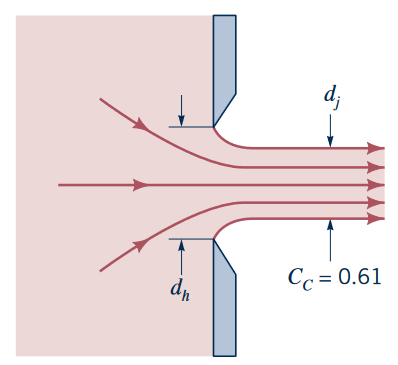
\includegraphics[width=0.5\textwidth]{Session_5/figs/vena_contracta}
    \caption{Picture from \cite{GerhartEtAl_20}.}
\end{figure}

We will work through a slightly different set-up called Borda mouthpiece where the coefficient of contraction could be obtained by hand. The Borda mouthpiece is a cylindrical tube, projecting inward to the center of the bucket.
\begin{figure}[H]
    \centering
    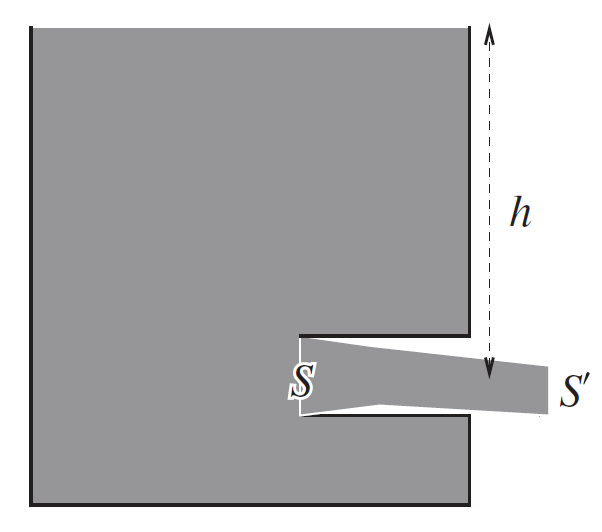
\includegraphics[width=0.4\textwidth]{Session_5/figs/borda}
\end{figure}
Name $S'$ the size of the jet area so that the coefficient of contraction is $S'/S$. 

\subsection{}
Assume $S'$ given, what is the discharge rate. What is the momentum flux of this discharge.

\subsection{}
We know that the horizontal momentum flux should be equal to a surface integral of the force from the wall of the bucket. Use this relation, and $v=\sqrt{2gh}$ to obtain the coefficient of contraction is $S'/S = 0.5$.

\section{Reynolds number for simple model for river flow}
[From \cite{Falkovich_18}, \S 1.4.3] 
We use a simple inclined plane as a model for river flow.
\begin{figure}[H]
    \centering
    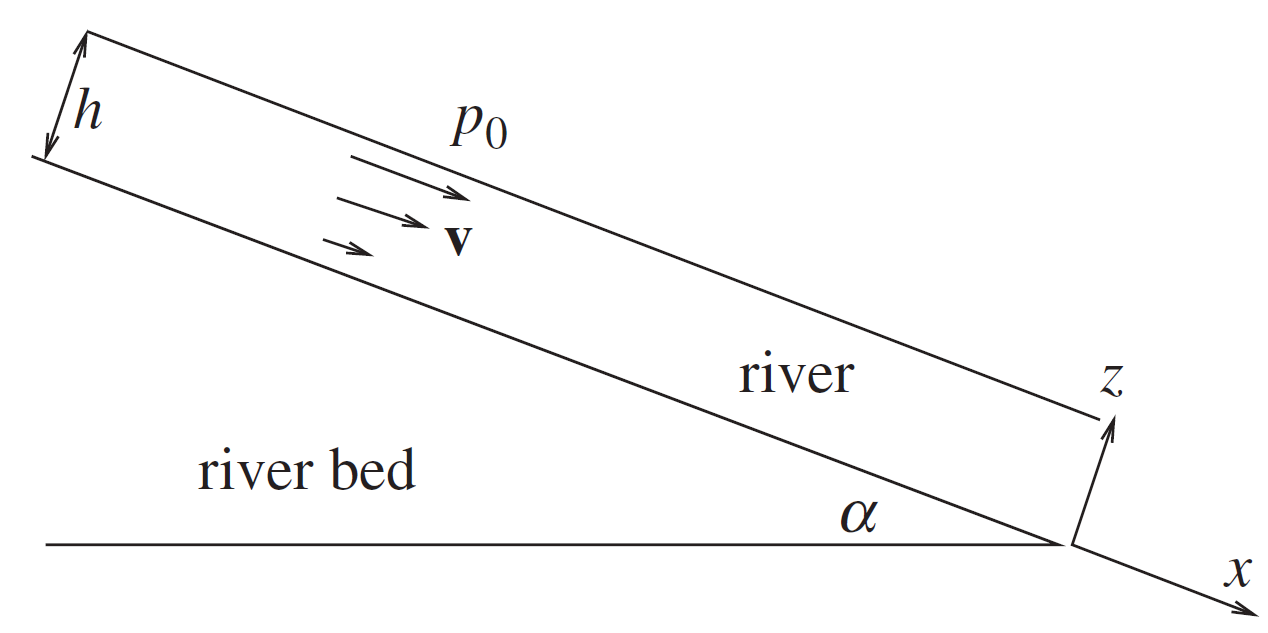
\includegraphics[width=0.55\textwidth]{Session_6/figs/incline_river}
\end{figure}

In lecture you have the obtained the solution of:
\begin{align}
    p(z) &= p_0+\rho g(h-z)\cos\alpha,\\
    v(z) &= \frac{\rho g\sin\alpha}{2\eta}z(2h-z).
\end{align}

\subsection{}
Take the kinematic viscosity of water to be $\nu = \eta/\rho = 10^{-2}\;\text{cm}^2\text{s}^{-1}$. Calculate $\ve v$ at the surface for a rain puddle with thickness $h = 1\;\text{mm}$ on a slope $\alpha\sim 10^{-2}$.

\subsection{}
How about a slow plain rivers (like the Danube) with $h \sim 10\;\text{m}$ on a slope $\alpha\sim 10^{-4}$?

\subsection{}
Which speed is reasonable?

\subsection{}
The unrealistic high velocity for the river case above is because in reality rivers are turbulent. Calculate the Reynolds number for the two cases.

\chapter{Vorticity Dynamics}
\section{Vorticity equation derivation}
Remember that we have the vector identity:
\begin{align}
    \ve v(\nabla\cdot\ve v) = \frac{1}{2}\nabla\ve v^2-\ve v\times\ve \omega.
\end{align}
To obtain the vorticity equation, we need to take the curl of this. 

\subsection{}
Derive the vector identity:
\begin{align}
    \nabla\times(\ve a\times\ve b) &= \ve a(\nabla \cdot \ve{b}) - \ve{b}(\nabla \cdot \ve{a})+(\ve{b} \cdot \nabla) \ve{a} \,-\, (\ve{a} \cdot \nabla) \ve{b}.
\end{align}
Hint: remember we have
\begin{align}
    \epsilon_{ijk}\epsilon_{k\ell m} = \delta_{i\ell}\delta_{jm}-\delta_{im}\delta_{j\ell}.
\end{align}

\subsection{}
Show that the compressible vorticity equation is
\begin{align}
    \frac{\pe\ve\omega}{\pe t}+(\ve v\cdot \nabla)\ve\omega = (\ve \omega\cdot \nabla)\ve v-\ve\omega\nabla\cdot\ve v
\end{align}
The incompressible version is an straightforward corollary. 

\section{Vorticity equation for compressible flows}
[From \cite{Vallis_17}, \S 4.2] Using mass-conservation for compressible flows:
\begin{align}
    \frac{\pe\rho}{\pe t}+\nabla\cdot(\rho\ve v) = 0
\end{align}
Obtain the alternative compressible vorticity equation:
\begin{align}
    \frac{\pe\tilde{\ve\omega}}{\pe t}+(\ve v\cdot \nabla)\tilde{\ve\omega} = (\tilde{\ve \omega}\cdot \nabla)\ve v
\end{align}
where
\begin{align}
    \tilde{\ve \omega} = \frac{\ve\omega}{\rho}.
\end{align}

\section{Fundamental solution to the heat equation}
For details, see \S 5.1 and 5.2 of \cite{ShearerLevy_15}.

\subsection{}
Self-similar solution from dimensional analysis. 

\subsection{}
Fundamental solution is the Green's function.

\section{Cylindrical coordinate}
Derivation I use is in \S5.1 and \S5.5 of \cite{Brannon_04}.

\section{Examples of vorticity and circulation}
When we deal with vorticity and circulation, it is most convenient to work with polar coordinate. In (2D) polar coordinate, the vorticity (scalar) is
\begin{align}
    \omega = \frac{1}{r}\left( \frac{\pe (ru^\theta)}{\pe r}-\frac{\pe u^r}{\pe \theta} \right).
\end{align}

\subsection{Rigid body rotation}
For a body in rigid body rotation, the velocity distribution is given by
\begin{align}
    u^\theta = \Omega r \qdt{and} u^r = 0
\end{align}
where $\Omega$ is the angular velocity of the fluid (rigid body). Calculate the vorticity of this flow. How is it related to the angular velocity?

\subsection{Rankine vortex}
We have the flow field
\begin{align}
    u^\theta = \begin{cases}
        \Omega r, & r<a\\
        \dsp{\frac{\Omega a^2}{r}}, & r\geq a
    \end{cases}
\end{align}
and $u^r = 0$. 
\begin{itemize}
    \item Calculate the vorticity of this flow.
    \item Calculate the circulation of this flow around a circle with radius $R$.
\end{itemize}

\subsection{Point vortex}
We take the $a\to 0$ limit of the Rankine vortex. For this, we define $K = \Omega a^2$ and keep this a constant as we take $a$ to zero. 
\begin{itemize}
    \item How does the vorticity change as we take $a\to 0$.
    \item What is now the circulation of this flow around a circle with radius $R>a$.
\end{itemize}

\section{Point vortex velocity as a Green's function}

\subsection{Biot–Savart law}
We have the velocity field around a single point vortex. Use this and the idea of Green's function to write down the velocity field for a vortex field. This is just the 2D Biot–Savart law relating vorticity and velocity.

\subsection{Green's function for the Poisson equation}
Incompressible flow can be represented using a streamfunction $\psi$, where\footnote{sometimes it is defined with the opposite sign}
\begin{align}
    (u,v) = (-\psi_y,\psi_x). 
\end{align}

\begin{itemize}
    \item Show that the streamfunction is the solution to the Poisson equation with the vorticity on the RHS:
        \begin{align}
            \nabla^2\psi = \omega.
        \end{align}
    \item Convert the Biot–Savart law to a streamfunction. This streamfunction of the Green's function for the Poisson equation. Now you could solve the Poisson equation in $\mathbb{R}^2$.
\end{itemize}

\section{Inviscid, incompressible vortex dynamics near a wall}
Now we study inviscid, incompressible flow in the upper half plane. At the wall we use the no penetration boundary condition:
\begin{align}
    v(0,y) = 0.
\end{align}

\subsection{}
Place a point vortex into the upper plane. 
\begin{itemize}
    \item How could we make sure the flow satisfies the boundary condition?
    \item Write this in the context of the Biot–Savart law.
\end{itemize}

Hint: try placing an imaginary point vortex in the lower half plane.

\subsection{}
Think about the flow using a streamfunction. 
\begin{itemize}
    \item What is the boundary condition on the streamfunction? 
    \item Write this using the Green's function formula for the solution of the Poisson equation.
\end{itemize}

\section{Two interesting and advanced vortices examples}
\subsection{Kirchhoff Vortex} Kirchhoff vortex is a compact elliptical patch of vorticity that rotate while keeping its shape. It is a generalization of the Rankine vortex and it is the basis of study of instability. 

For details of the Kirchhoff Vortex, see \url{http://www.damtp.cam.ac.uk/user/hl278/KirchoffVortex.pdf}. For an example study of its stability, see \cite{MitchellRossi_08}.

\subsection{Lamb–Chaplygin dipole} The Lamb–Chaplygin dipole has also compact vorticity but it has positive and negative vorticity inside. It is a steady solution to the Euler equation. For more see \cite{MeleshkoHeijst_94}, image above from wikipedia.
\begin{figure}
    \centering
    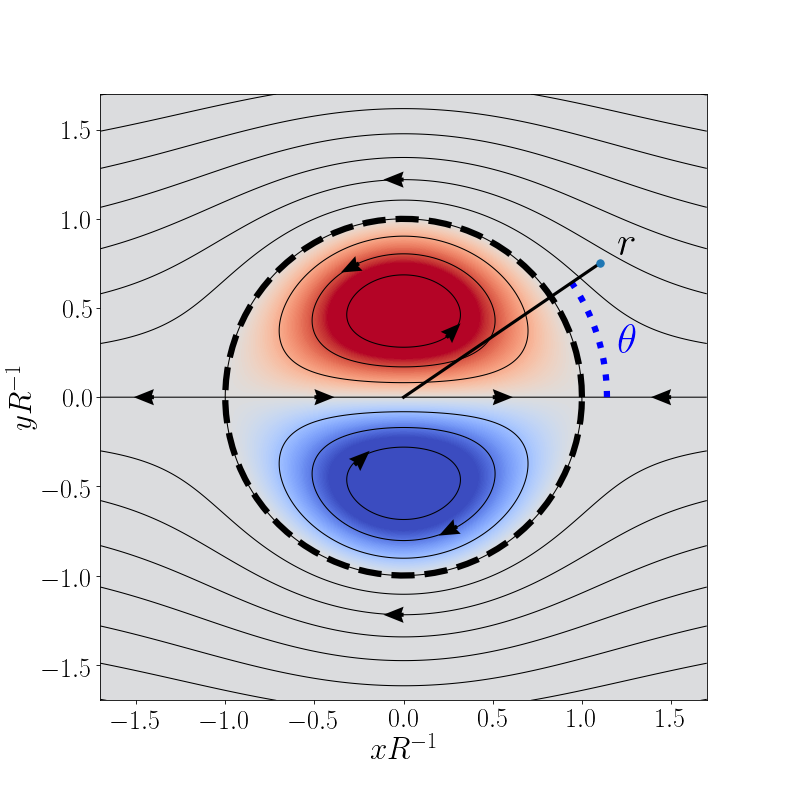
\includegraphics[width = 0.5\textwidth]{../Session_8/figs/Lamb-Chaplygin_dipole}
\end{figure}

\chapter{Potential Flow}
\section{Helmholtz decomposition}
The Helmholtz decomposition state that a velocity field $\ve v$ that decays fast enough at infinity, or is on a bounded domain, can be decomposed into a curl-free component and a divergence-free component \parencite{Petrascheck_15}
\begin{align}
    \ve v = -\nabla\Phi+\nabla\times \ve A. 
\end{align}

\subsection{}
Show that this is a generalization of the 2D situation where we have scalar potential and stream functions. 

\subsection{}
How would you find these two potentials if you know the divergence and vorticity in the domain?

\section{Baby steps in complex analysis. }
We will learn a little bit of complex analysis. My reference is \cite{SteinShakarchi_10}. 

\section{Bernoulli's theorem for irrotational flow}
Because the velocity can be expressed as the gradient of a potential, now the fluid can be unsteady. 

\chapter{Instability}
\section{Kelvin-Helmholtz instability}
We will investigate the Kelvin-Helmholtz instability from a Fourier mode perspective. The reference I will use is \S9.2 of \cite{Vallis_17}.

\section{Centrifugal instability}
A circular patch of vorticity can be unstable too. We will replicate some of the procedure for the study of Kelvin-Helmholtz instability to circular vortex patch. The reference is \S 3.3 of \cite{McWilliams_06}.

\chapter{Stokes Flow}
\section{Pressure is a Lagrange multiplier for incompressible flow}
We have talked about how pressure is a Lagrange multiplier that enforces incompressibility. This is the easier to show for Stokes flow. Show that the Stokes equation on $\Omega$
\begin{align}
    &-\mu\lap \ve u + \nabla p = f\\
    &\qquad \left.\ve u\right|_{\pe\Omega} = 0\\
    &\qquad\nabla\cdot \ve u = 0
\end{align}
is equivalent to a constrained energy minimization problem:
\begin{align}
    &\min_{\ve u} \frac{\mu}{2}\int_\Omega \norm{\nabla\ve u}^2-f\ve u\;\de \ve x\\
    &\text{subject to }\nabla\cdot \ve u = 0.
\end{align}

\section{Uniqueness of solution for Stokes}
Show that the solution to the Stokes system is unique from the energy minimizing statement above. This is a similar but slightly different approach compared to the one in \cite[\S 7.4]{Acheson_90}. 

\section{Life at low Reynolds number}
If we have time left, we will take a look at the classic and highly readable paper \cite{Purcell_77}. Life at low Reynolds number is counter-intuitive and full of surprise.



\newpage
\printbibliography

\end{document}